% !TEX root = ../thesis.tex
Beryllium metal is ablated with an Nd:YAG laser and trapped in a linear Paul trap. Laser cooling is applied with a 313nm laser. Pure O$_2$ gas is introduced into the chamber via leak valve to react with the ions. Remaining reactants and charged reaction products are ejected into a time-of-flight mass spectrometer (TOF) where the various masses of ions can be determined.

When the Be$^+$ is excited from the $^2$S$_{1/2}$ to the $^2$P$_{3/2}$ manifold, we find the energetically allowed channels to be:

\begin{align}
    \text{Be}^+(^2\text{P}_{3/2}) + \text{O}_2 & \to \text{O}_2^+ + \text{Be} \label{eq: o2+} \\
    & \to \text{BeO}^+ + \text{O}_2 \label{eq: beo+} \\
    \text{Be}^+(^2\text{P}_{3/2}) + \text{H$_2$O} & \to \text{BeOH}^+ + \text{H} \\
    \text{Be}^+(^2\text{P}_{3/2}) + \text{H}_2 & \to \text{BeH}^+ + \text{H} \\
    \text{BeH}^+ + \text{H$_2$O} & \to \text{BeOH}^+ + \text{OH}
\end{align}

Without excitation into the $^2$P$_{3/2}$ manifold, reactions \ref{eq: o2+} and \ref{eq: beo+} are endothermic by 2.75eV and 1.1eV, respectively.

Despite the fact that reaction \ref{eq: beo+} is energetically allowed, it is never seen with laser cooling.

Without 313nm light, the Be$^+$ ions stay in the $^2$S$_{1/2}$ ground state, but with a ion trap depth > 4eV, there are portions of the ion cloud with enough energy to still proceed with the production of BeO$^+$. Without the laser cooling, we observe the disappearance of BeO$^+$ from the trap due to exciting the molecule into a pre-dissociative state.

\begin{figure}[H]
	\centering
	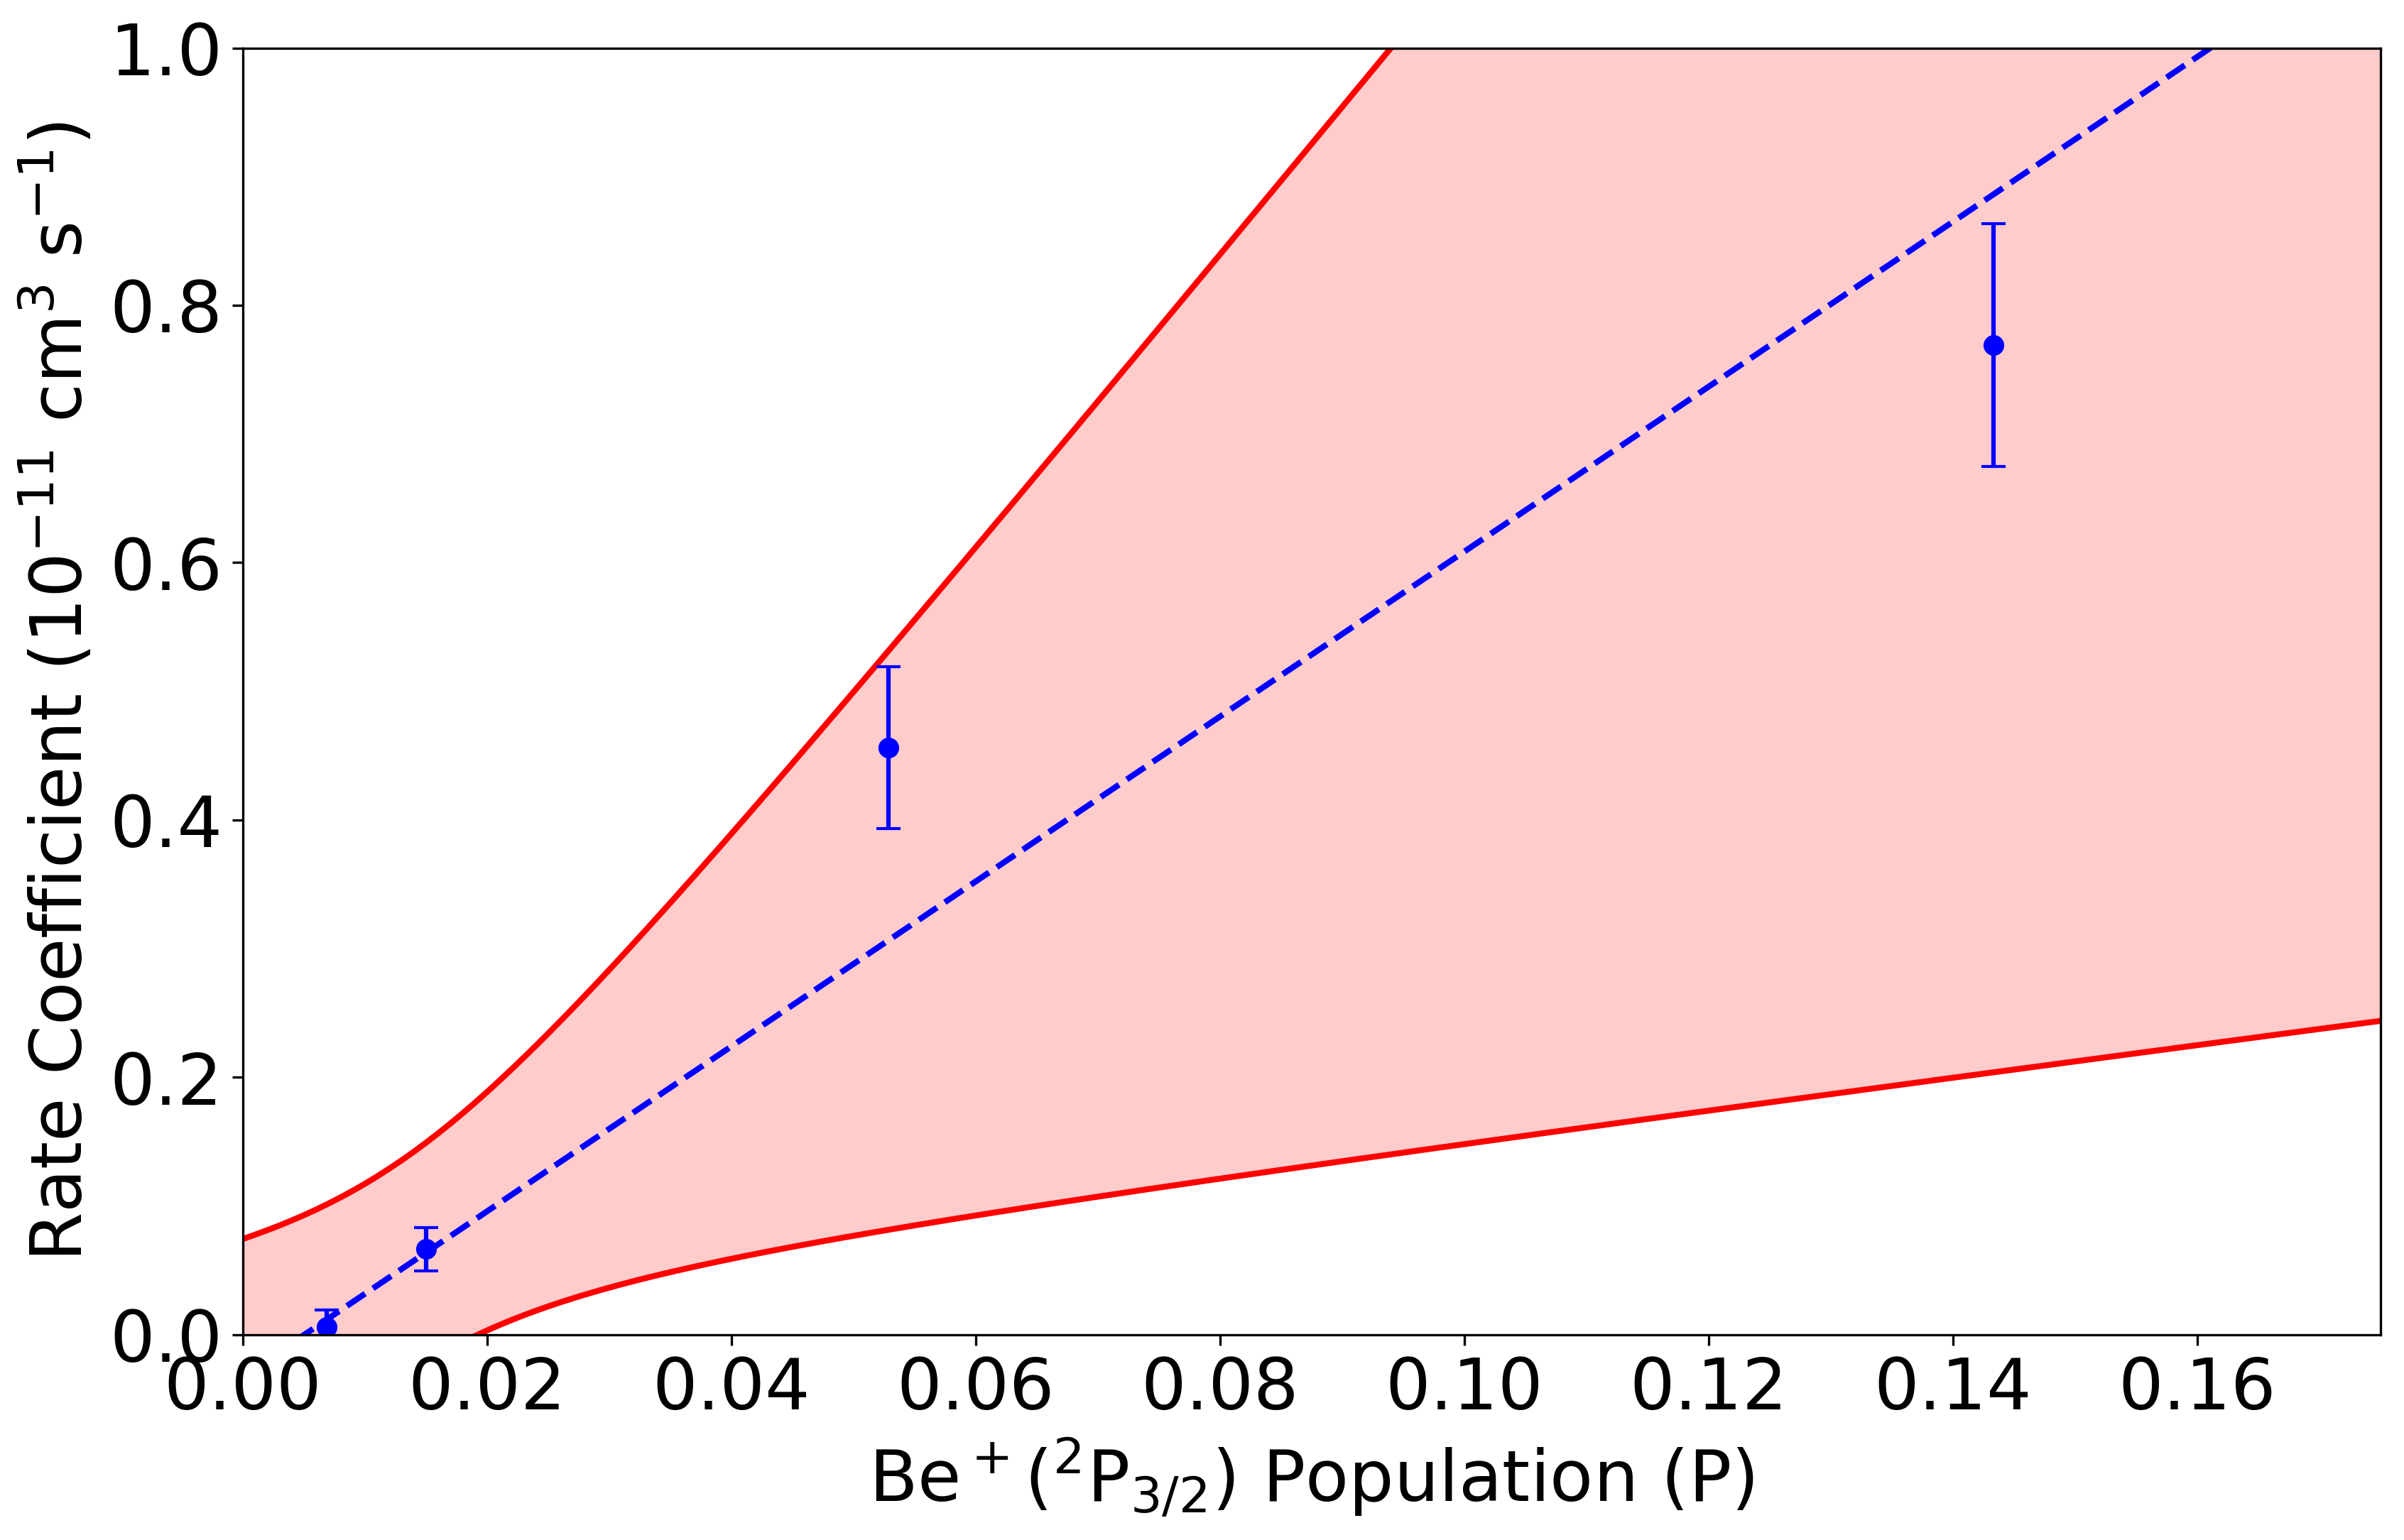
\includegraphics[width=0.7\textwidth]{images/Be_O2_P_state.png}
	\caption{\label{fig: p-state} A linear dependence on the rate constant for reaction \ref{eq: o2+} as a function of P state excitation. $k = (6 \pm 1) \times 10^{-11} P + (-0.03 \pm 0.16) \times 10^{-11}$}
\end{figure}

% \begin{figure}[H]
%	 \centering
%	 \includegraphics[width=0.5\textwidth]{p_state_no_b.png}
%	 \caption{\label{fig: p-state} A linear dependence on the rate constant for reaction \ref{eq: o2+} as a function of P state excitation. Fit $(5.45 \pm 1.03) \times 10^{-11} P$}
% \end{figure}

\begin{figure}[H]
	\centering
	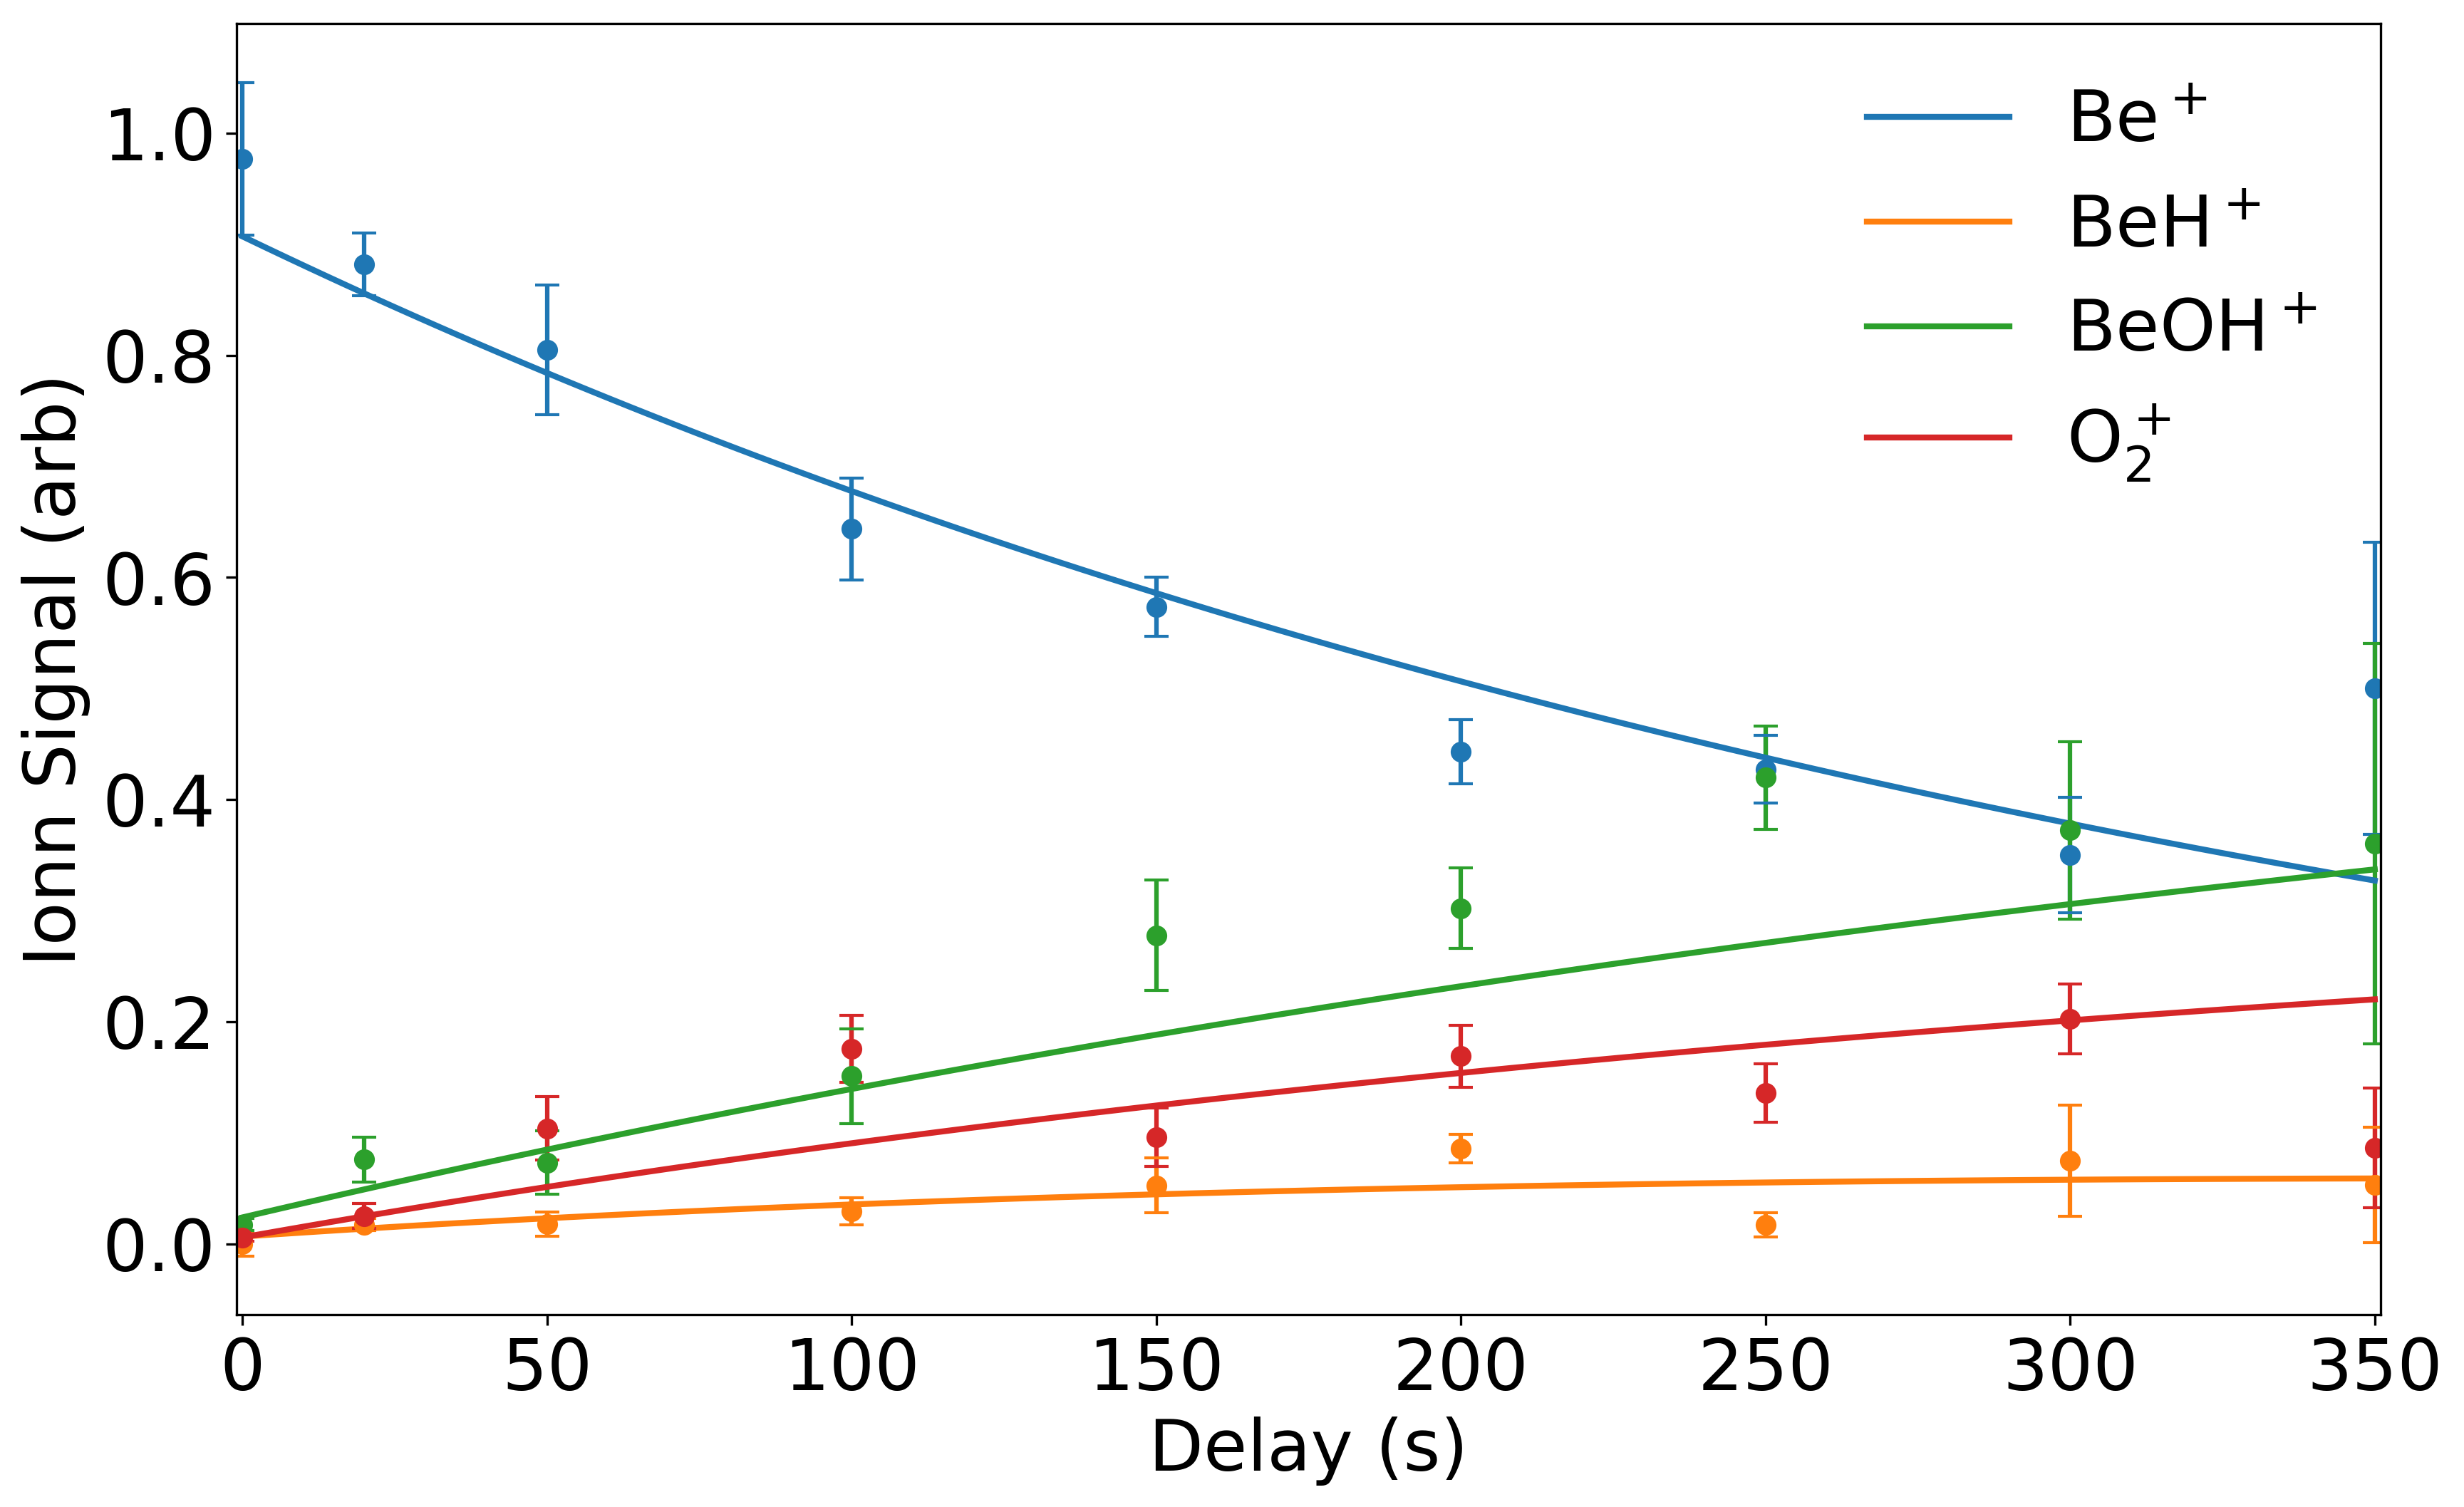
\includegraphics[width=0.7\textwidth]{images/Be_O2_laser_fit.png}
	\caption{\label{fig: laser fit} Shared fitting of trapped products with 14\% p-state excitation.}
\end{figure}

\begin{figure}[H]
	\centering
	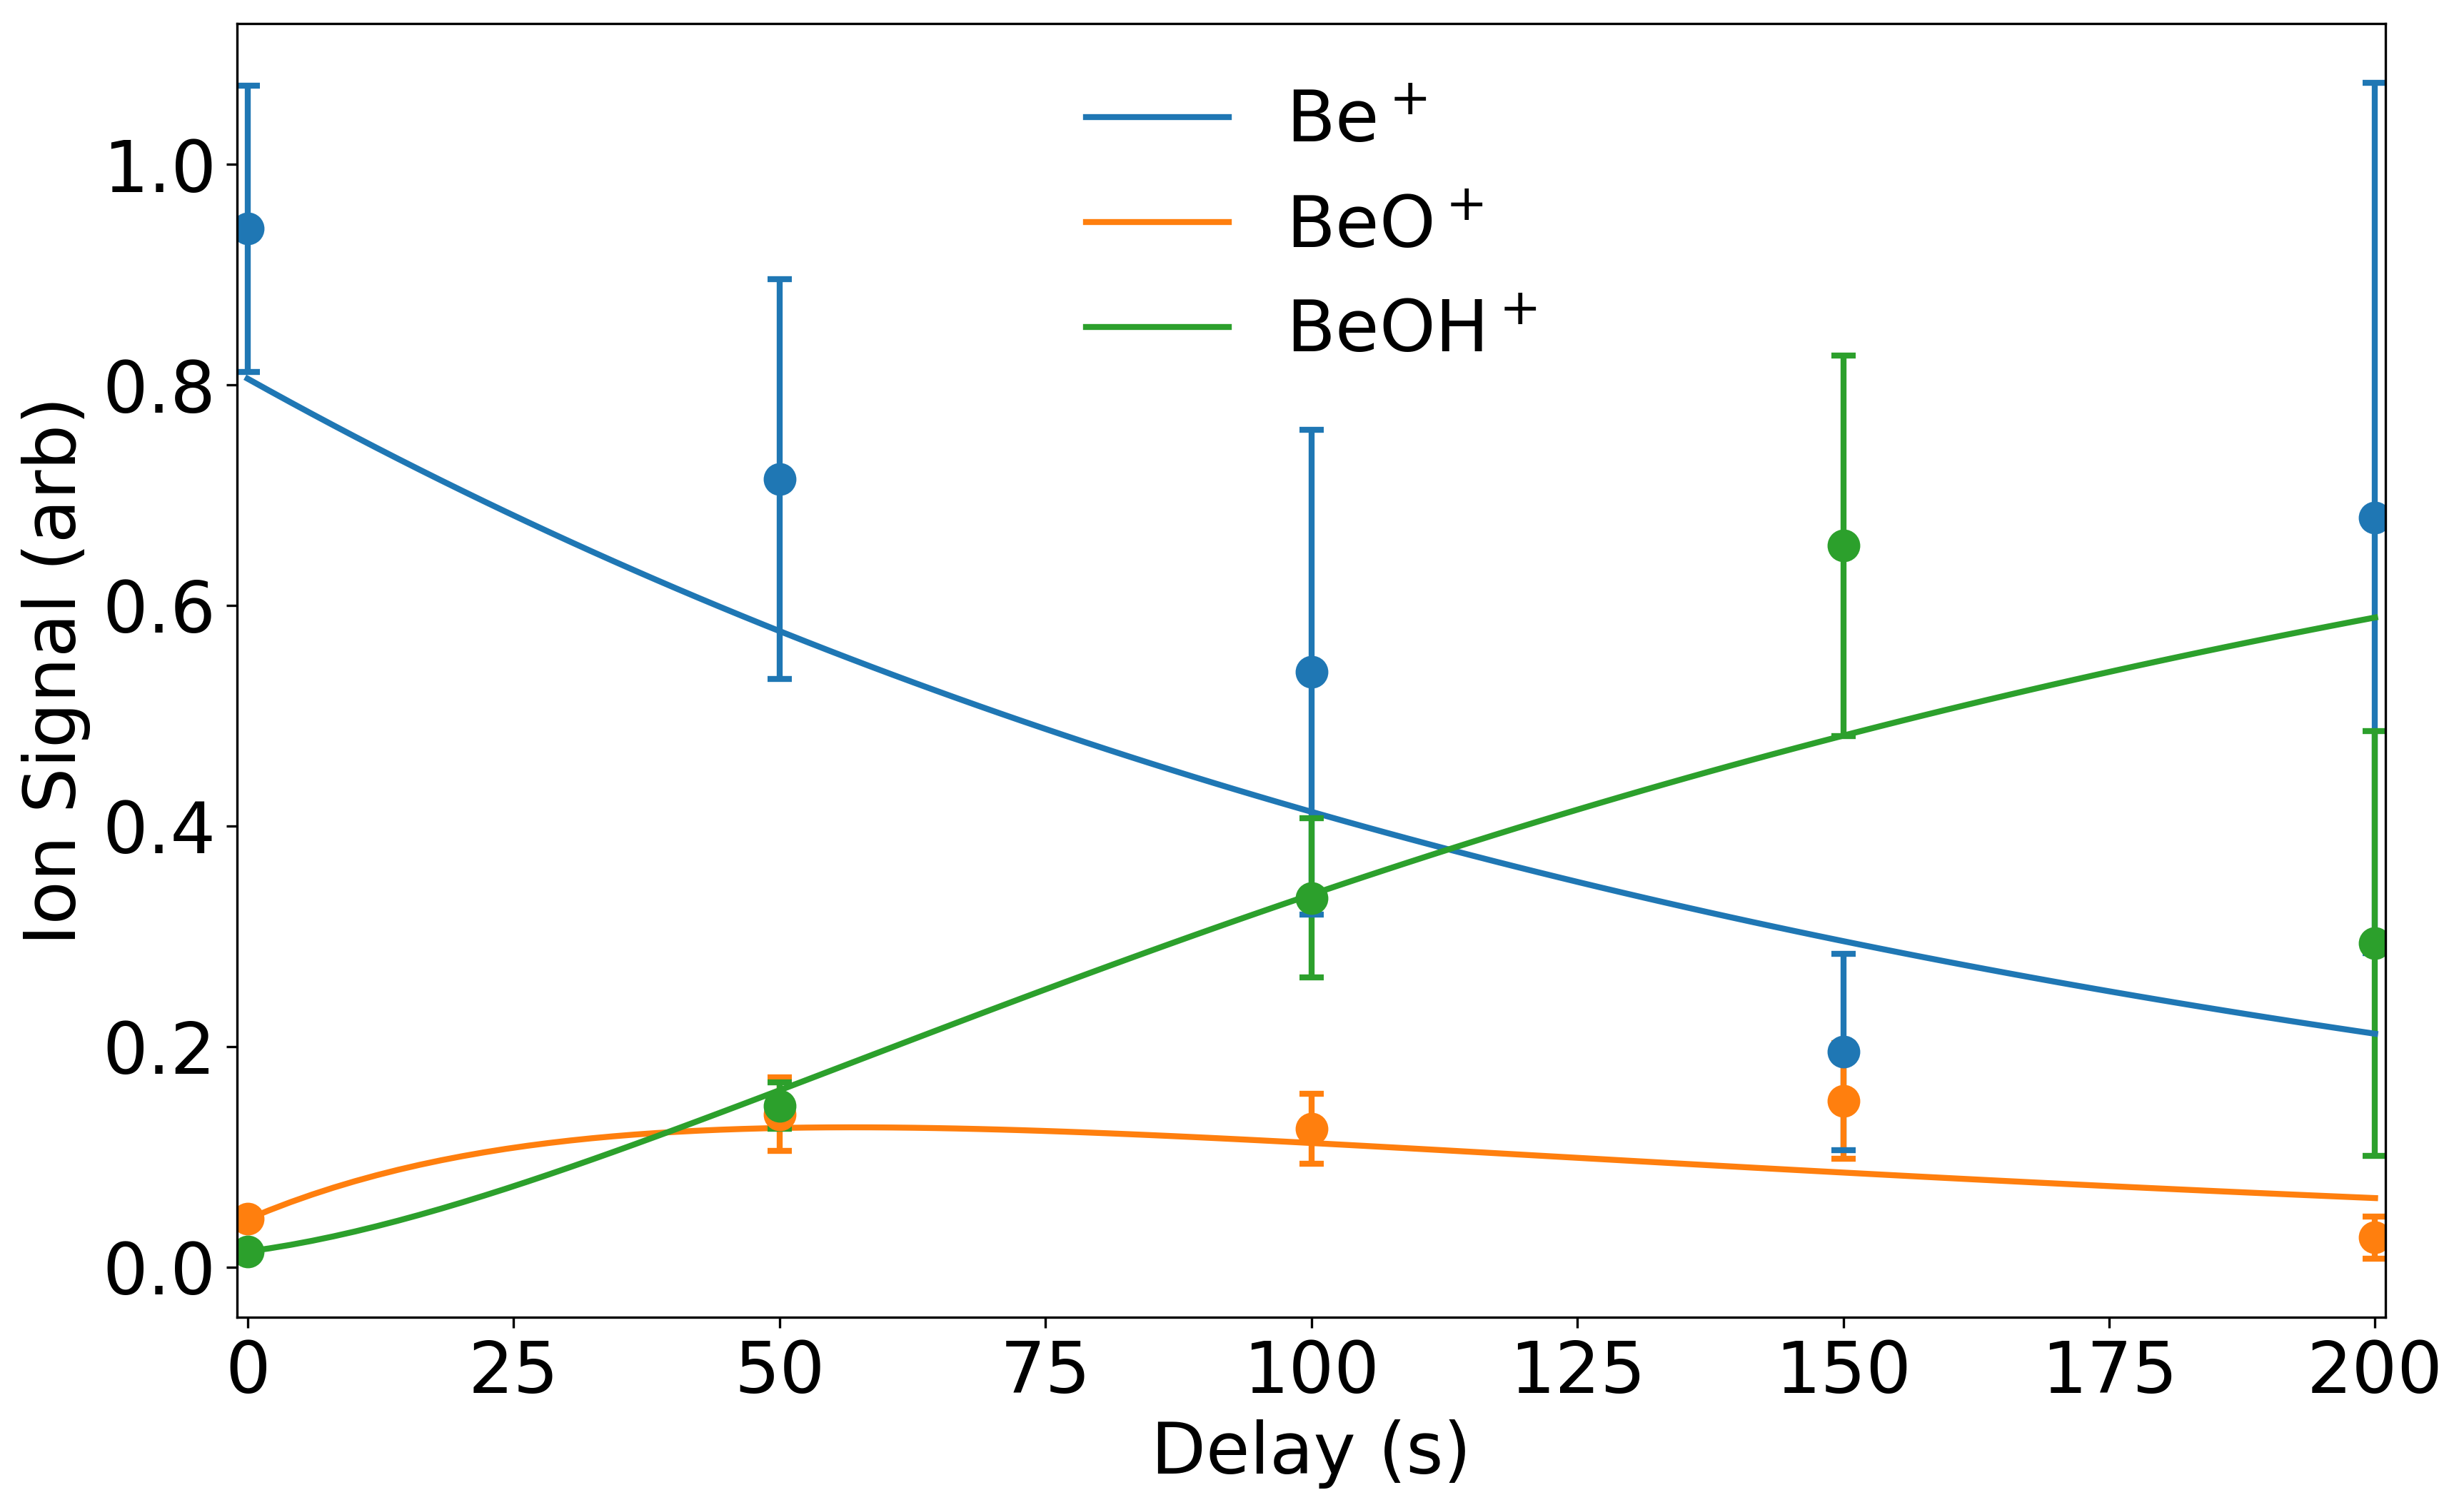
\includegraphics[width=0.7\textwidth]{images/Be_O2_no_laser_fit.png}
	\caption{\label{fig: no laser fit} Shared fitting of trapped products with 14\% p-state excitation.}
\end{figure}

\begin{figure}[H]
	\centering
	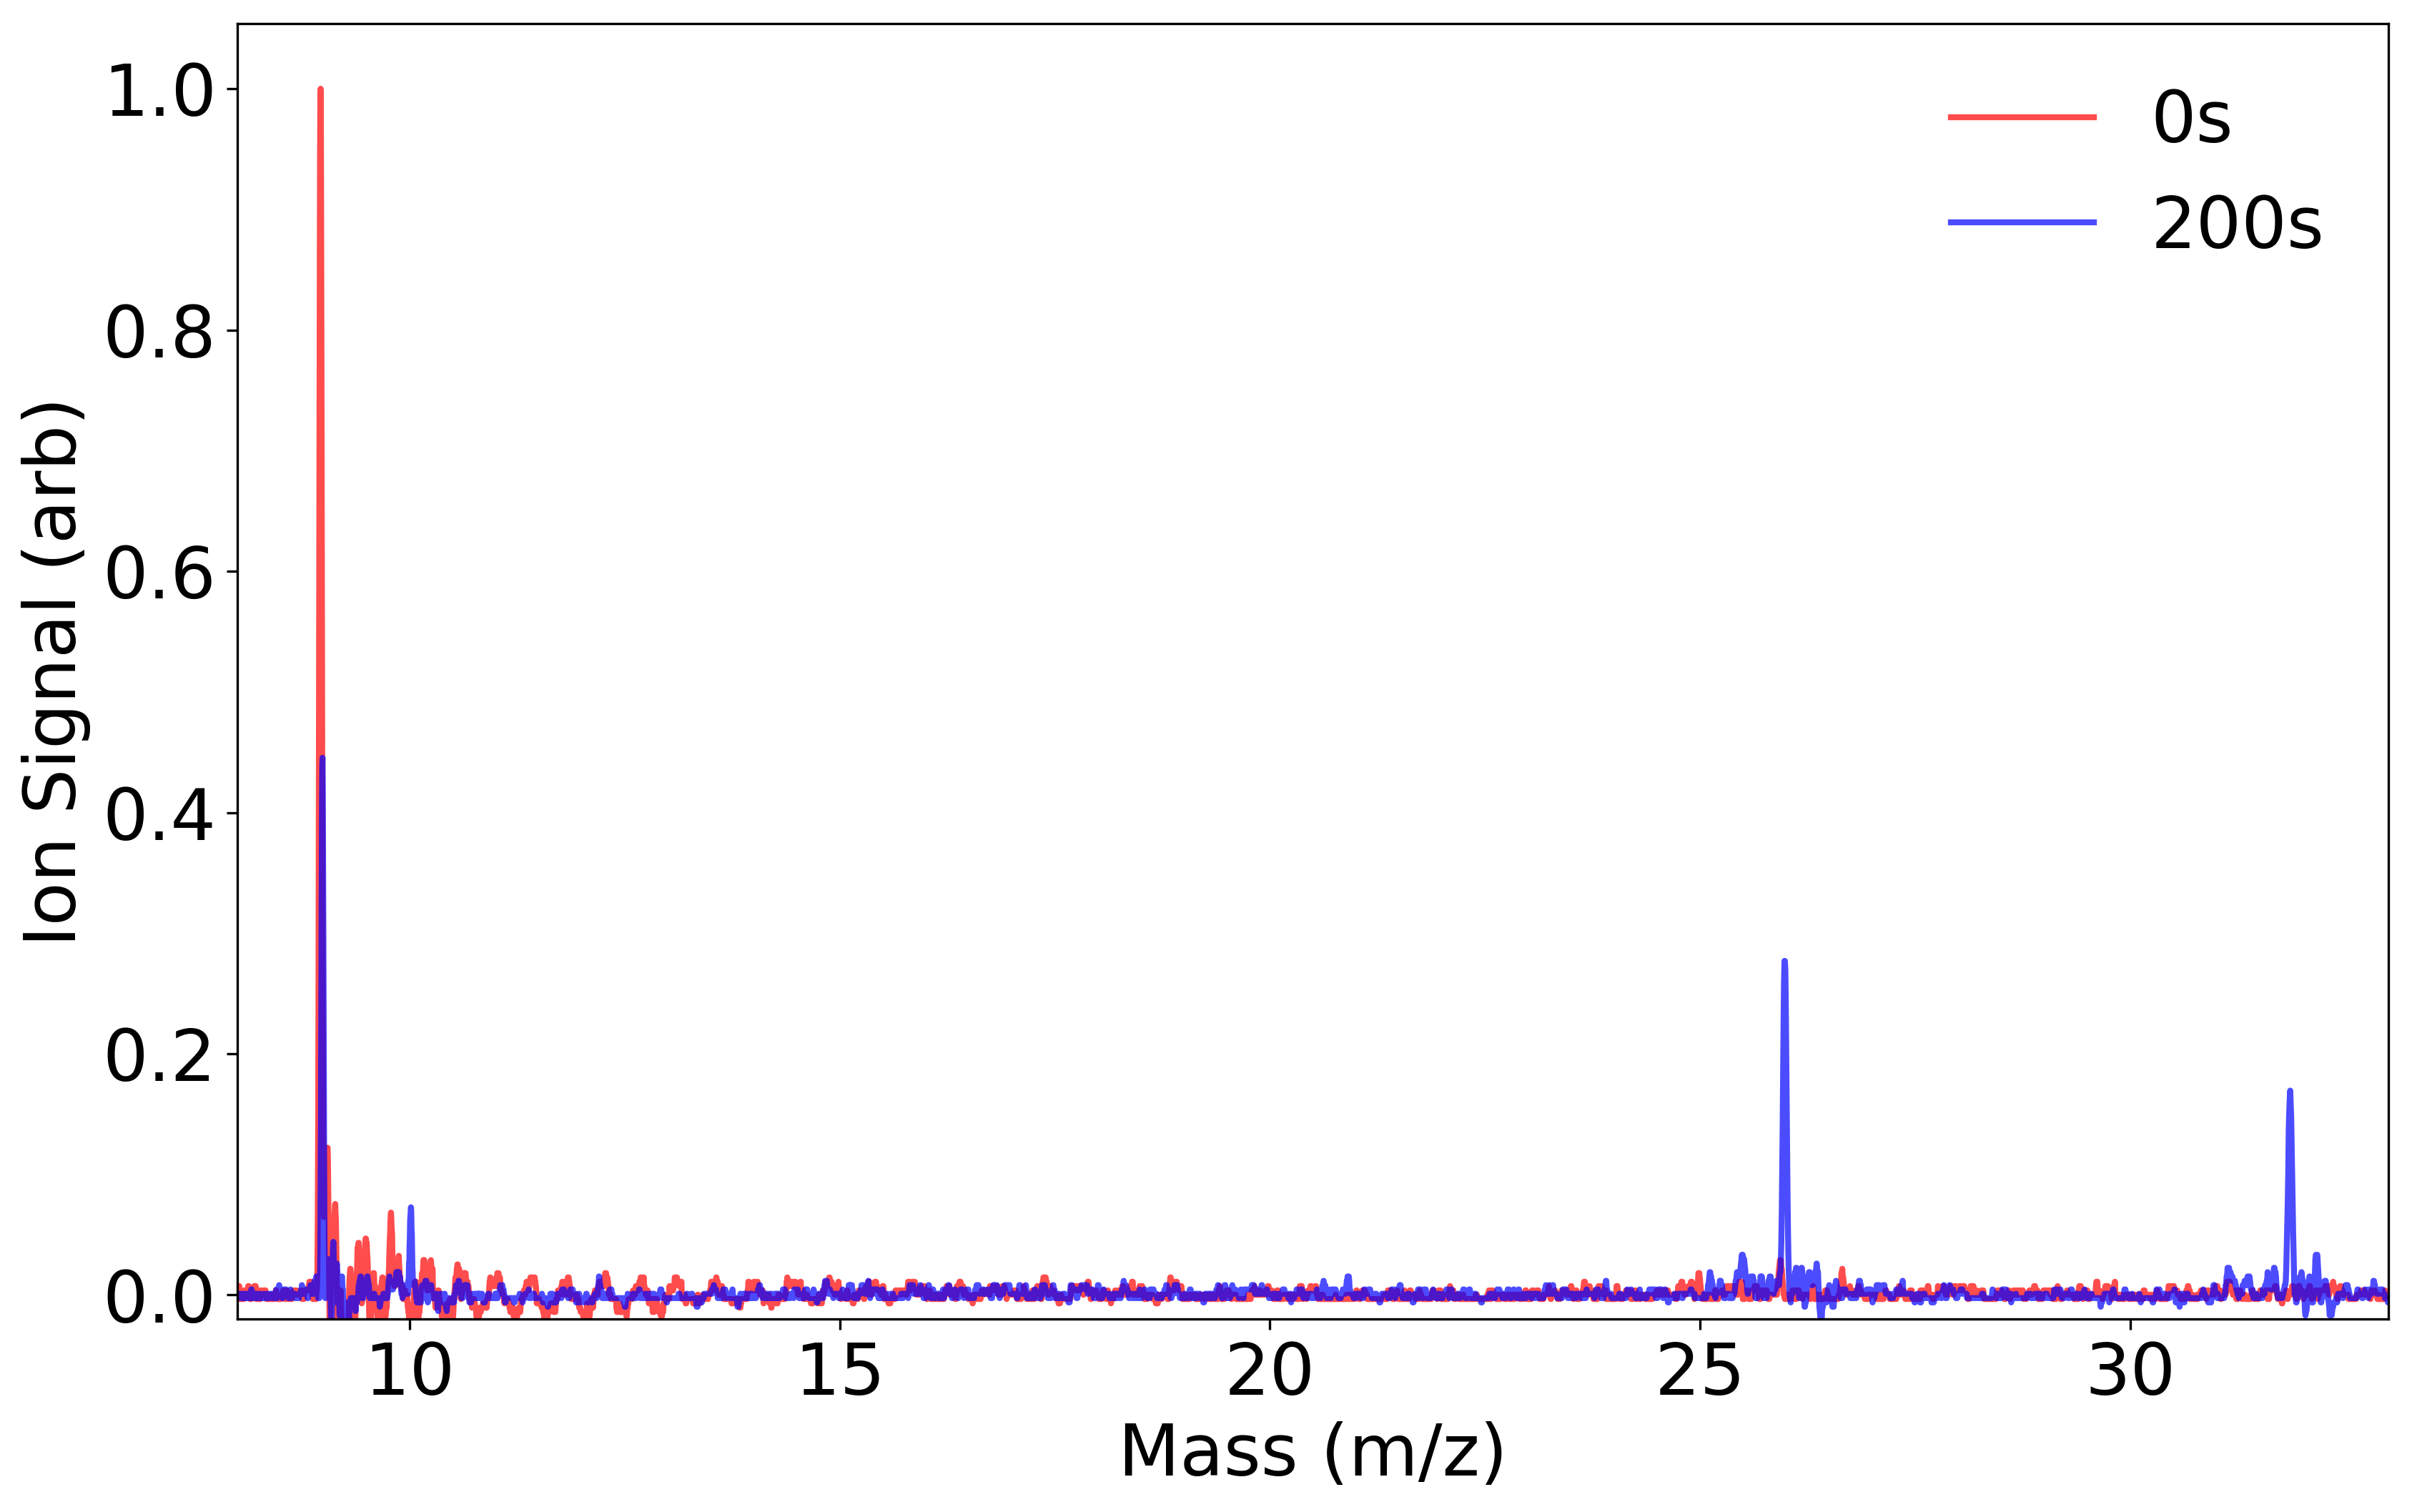
\includegraphics[width=0.7\textwidth]{images/Be_O2_laser_TOF.png}
	\caption{\label{fig: laser TOF} TOF traces for data taken with 14\% p-state excitation at 0s and 200s showing no products at 0s, but distinct peaks for reaction products BeH$^+$, BeOH$^+$, and O$_2^+$.}
\end{figure}

\begin{figure}[H]
	\centering
	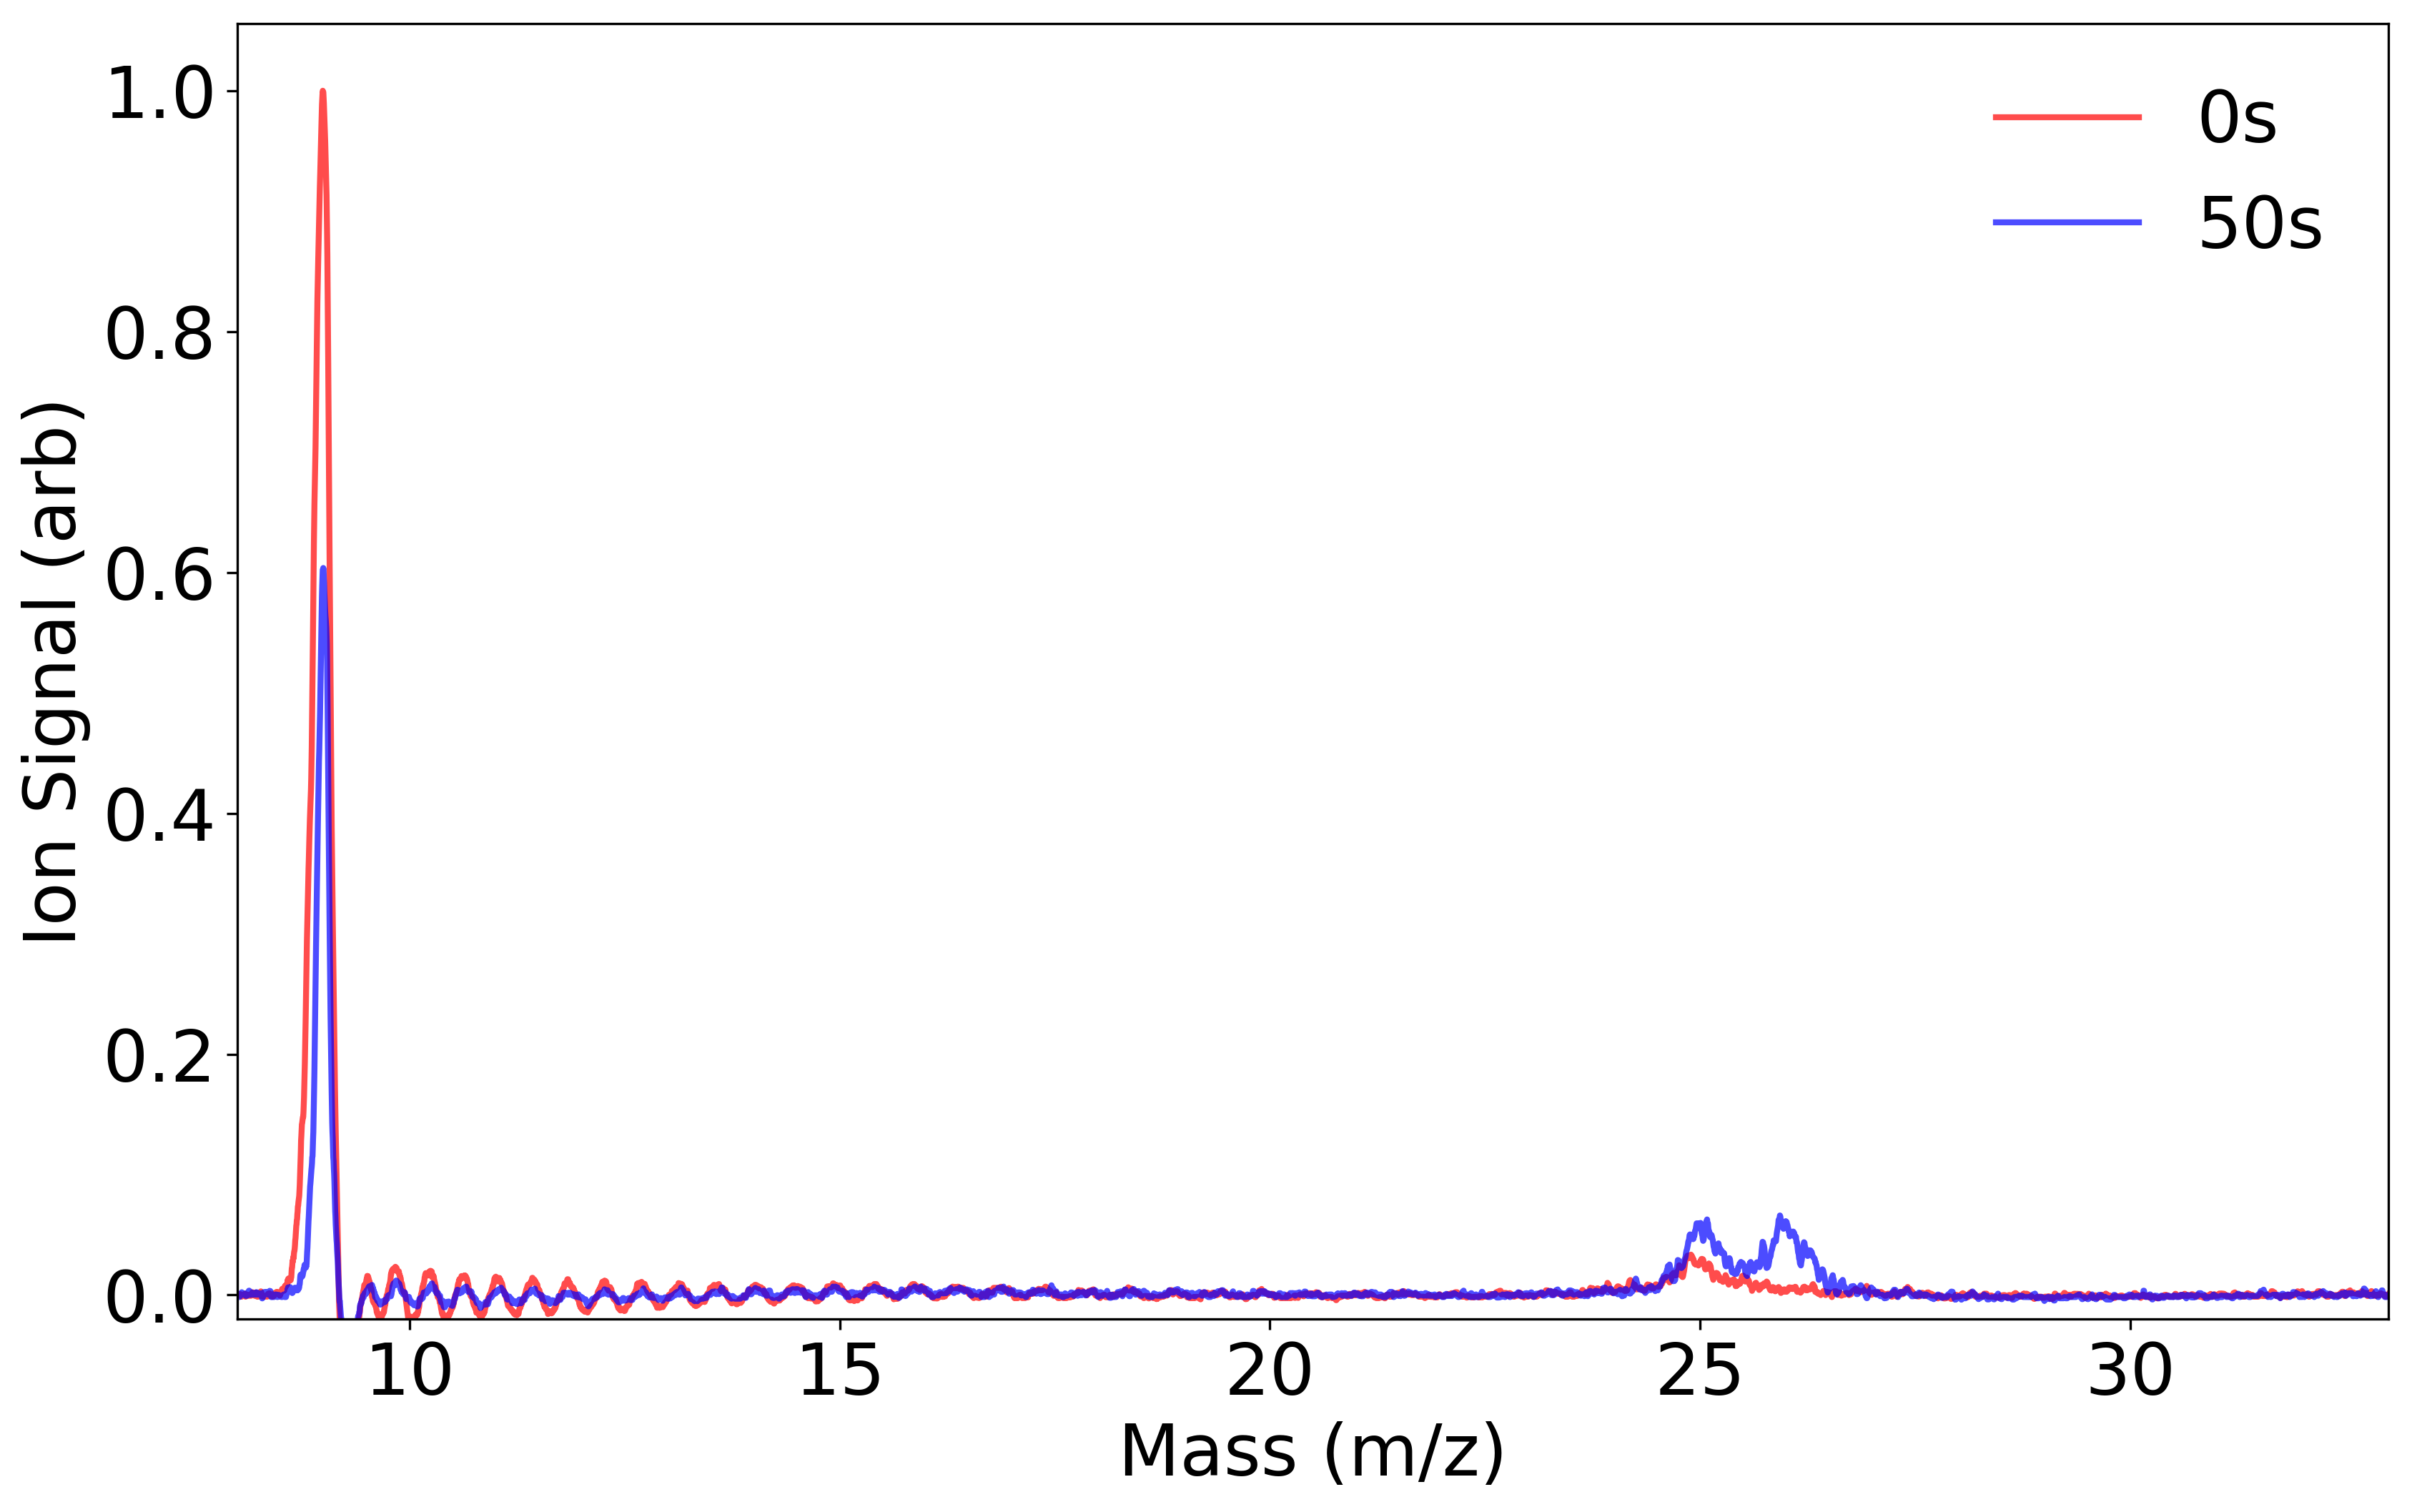
\includegraphics[width=0.7\textwidth]{images/Be_O2_no_laser_TOF.png}
	\caption{\label{fig: non laser TOF} TOF traces for data taken with 14\% p-state excitation at 0s and 200s showing no products at 0s, but distinct peaks for reaction products BeH$^+$, BeOH$^+$, and O$_2^+$.}
\end{figure}

Considering state counting, reactions \ref{eq: co} and \ref{eq: o} have been measured to have branching ratios that vary from 60:40 (CO$^+$:O$^+$) to 30:70 in the other direction. By looking at experimental data as well as the theoretical state counting, we find the ratio to be pretty definitively 60:40.
